\title{311 Home Work 1}
\author{
   Ben purdy
}
\date{\today}

\documentclass[12pt]{article}
\usepackage{tikz-qtree}

\usepackage{algorithmic}
\usepackage[utf8]{inputenc}
\usepackage[english]{babel}
\newtheorem{theorem}{Theorem}
\usepackage{algorithmic}
\usepackage[noline,ruled,noend]{algorithm2e}
\setlength{\algomargin}{7.5pt}
\usepackage{amssymb}
\usepackage{amsmath}
\usepackage{amsthm}
\begin{document}
\maketitle
\tikzset{every tree node/.style={minimum width=2em,draw,circle},
         blank/.style={draw=none},
         edge from parent/.style=
         {draw,edge from parent path={(\tikzparentnode) -- (\tikzchildnode)}},
         level distance=1.5cm}

\section{}
 An alternative method of performing an tree walk of an inorder n-node binary search tree finds the minimum element in the tree by calling Minimum and then making  $n-1$ calls to Successor. Analyze this algorithm, and show that it runs in$ \Theta(n)$ time.\\
 tree walk is O(n)
 
 	\begin{proof}
 	
 	By calling successor n-1 time after calling minimum once running in O(h). This will start at the leftmost node of the tree propagate up to its parent by the first successor call. At the parent, this will go right and then down the leftmost subtree. repeating this action will visit all nodes in the tree. At worst all nodes will be visited on the way down and on the way up. Since all nodes will be visited and at most twice. This means that the running time is twice the number of edges. $2(nodes -1)\Rightarrow O(n^2)$, and $\Omega(n)$ because each node is visited once. 
 	
 	hence $\Theta(n)$.
 	\end{proof}
	
	\pagebreak 
 
 	\section{}
 We can sort a given set of n numbers by first building a binary search tree containing these
numbers (using Insert repeatedly to insert the numbers one by one) and then printing the
numbers by an inorder tree walk.
(a) What are the worst-case and best-case running times for this sorting algorithm if we
use an ordinary binary search tree? Justify your answer.
(b) Suppose that, instead of an ordinary binary search tree, we use a red-back tree. What
are the worst-case and best-case running times for this sorting algorithm? Justify your
answer.\\

Trivially inorder tree traversal is O(n). 

 	\begin{proof}  -  Justification 
 
 	(a)	
 	
The worst-case for insertion in an ordinary binary tree in (ascending/descending) order creating a list extending to the right/left of the head node. When building the binary tree, since it is a list each iteration takes the hight time. So with n nodes $(\sum_{k=0}^n = \frac{n(n+1}{2}$). Thus the run time is $O(n^2)$
 	
 	The best case. If the binary tree is balanced then insertion takes O(h). For any size balanced binary tree insertion still takes O(h). The hight of the tree cant exceed log(n) depth, thus for adding n nodes insertion takes O(nlog(n))
 	
	(b). 
	
	Worst case. red-black trees are balanced binary search trees. This means that insertion takes O(h) = O(log(n)). Since a red-black tree can only be balanced the worst case for insertion is $O(nlog(n))$. 
	"also see RBinsert run time proof from RB Trees-1.pdf"
	
	Best case. Insertion takes O(logn) because its balanced. to insert n nodes into a full binary tree takes O(nlogn). 
	see reasoning for above in (a) bestcase and (b) worst case
	
	red-black trees are balanced binary search trees that guarantee tha tall query (Search,Maximum, etc.)  and update (Insert and Delete)operations takeO(logn)time in the worst case.
 
 	\end{proof}
 
 	\section{}
 Suppose that instead of each node x keeping the attribute x.parent, pointing to x’s parent, it keeps x.successor, pointing to x’s successor. Give pseudocode for Search, Insert, and Delete on a binary search tree T using this representation. These procedures should operate in time O(h), where h is the height of the tree T, and should update successor fields as necessary. Consider only ordinary binary search trees, not red-black trees. (Hint:
You may wish to implement a subroutine that returns the parent of a node.)\\\\

assume for the deletion procedure that all the keys are distinct, as
that has been a frequent assumption throughout this chapter. This will however
depend on it. Our deletion procedure first calls search until we are one step away
from the node we are looking for, that is, it calls Predecessor( Root T,key)

\begin{algorithm}[H]
Successor(tree T,node  x)\\
  \If{right[x] != null}{
    return minimum(right[x])\\
    }
  \Else{
    return TreeSuccessor(root[T], x, NIL)\\
    }

TreeSuccessor(y, x, c)\\
  \If{y = x}{
    return c\\
    }
  \If{key[x] $<$ key[y]}{
    return TreeSuccessor(left[y], x, y)\\
  }
  \Else{
    return TreeSuccessor(right[y], x, c)\\
	}

\end{algorithm}

%+================================ 	
\begin{algorithm}[H]
INSERT(T, z)\\
    y = NIL\\
    x = T.root\\
    pred = NIL\\
    \While{ x != null}{
        y = x\\
     }
        \If{z.key $<$ x.key}{
            x = x.left\\
         }
        \Else{
            pred = x\\
            x = x.right\\
        }
    \If{y == null}{
        T.root = z\\
        z.succ = NIL\\
     }
    \ElseIf{ z.key $<$ y.key}{
        y.left = z\\
        z.succ = y\\
        \If{pred != null}{
            pred.succ = z\\
        }
    }
    \Else{
        y.right = z\\
        z.succ = y.succ\\
        y.succ = \\
        }
\end{algorithm}
%+================================

\begin{algorithm}[H]
comment == how is this wrong. I got scared and left it.
Insert(treeRoot T,node  x)
\If{T == null}{
	T = x\\
	return\\
}
\If{x $<$ T}{
	return Insert( T.left,x);
}
\ElseIf{x $>$ T}{
	return Insert( T.right,x);
}
return T;\end{algorithm}

\begin{algorithm}[H]
Predecessor(value x, key k)
	\If{ k $<$ x.key}{
	y = x.left\\
	}
	\Else{y = x.right\\}
	\If {y == NIL}{
	throw error
	}
	\ElseIf{ y.key = k}{
	return x
	}
	\Else{}{
	return Predecessor(y,k)
	}
\end{algorithm}


 %+================================	
 
 	\section{}
What is the largest possible number of internal nodes in a red-black tree with black-height k? What is the smallest possible number? Express your answer as a function of k.\\


black hight for 2 example\\\\
  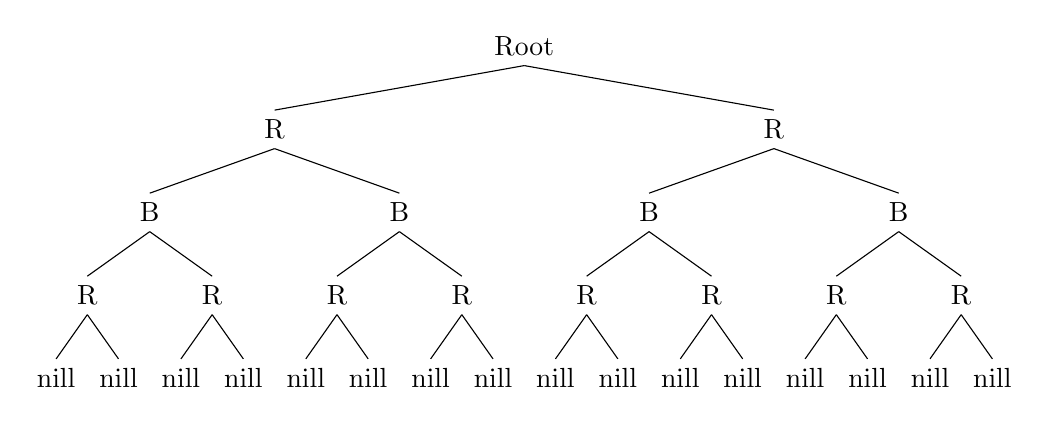
\begin{tikzpicture}
\Tree
[.Root     
    [.R  
    	[.B 
    		[.R [.nill ][.nill ]
    		]
    		[.R [.nill ][.nill ]
    		]
    	] 
    	[.B 
   			[.R [.nill ][.nill ]
   			]
   			[.R [.nill ][.nill ]
    		]
   		]
    ]	
    [.R  
   		[.B 
   			[.R [.nill ][.nill ]
   			]
   			[.R [.nill ][.nill ]
    		]
   		]
   		[.B 
   			[.R [.nill ][.nill ]
   			]
   			[.R [.nill ][.nill ]
    		]
   		]
   	]
]
\end{tikzpicture}

\pagebreak


 			\begin{equation}
 	 			a_1 = \sum_{n=0}^{2k-1}2^n = 4^k -1 = 2^{2k}-1
 			\end{equation} 
 			 			
the root is counted as a internal node and the largest number of internal nodes behaves on the summation $a_1$ becuase  by starting with red nodes after the root you have to double the hight adding k more rows. The by adding k more rows and removing the external nill nodes you get 2k-1 for your internal hight. 
 	
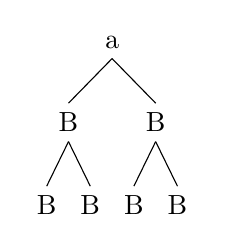
\begin{tikzpicture}
\Tree
[.a     
    [.B  
    	[.B ] [.B ]]
    [.B  
    	[.B ] [.B ]]
]
\end{tikzpicture}

 			\begin{equation}
 	 				a_2 = \sum_{n=0}^{k-1}2^n = 2^k -1
 			\end{equation}  			
 			the smallest case is $a_2$ becuase if the tree is compitly black the number of nodes is $a_2$. After you remove the nill nodes you get k-1 hight of external nodes



 	
 
 	\section{}
  
  A d-ary heap is like a binary heap, but (with one possible exception) non-leaf nodes have
d children instead of 2 children.\\
	\pagebreak
(a) How would you represent a d-ary heap in an array?\\

A d-array heap will behave the same way as a normal heap but you add d children behind the parent node.\\

parent(index i) = {(i-1)/d} -- this returns the parent position\\
child(index i , j jth child) = j+di+1 -- this returns any child position for any nodes parent.

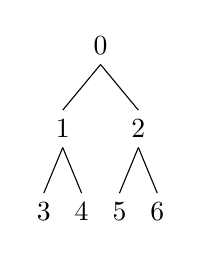
\begin{tikzpicture}
\Tree
[.0     
    [.1  
    	[.3 ] [.4 ]]
    [.2  
    	[.5 ] [.6 ]]
]
\end{tikzpicture}

(b) What is the height of a d-ary heap of n elements in terms of n and d? Justify your answer.
A-ary heap would have a height of S $\Theta(log_dn)$ We know that
		
		\begin{equation}
 	 		n = \sum_{i=0}^{h}d^i	 = \frac{d^{h+1}-1}{d-1}
 		\end{equation} 
	
	\begin{align*}
	n &= \frac{d^{h+1}-1}{d-1}\\
	n(d-1) &= d^{h+1}-1\\
	n(d-1)+1 &= d^{h+1}\\
	log_d(n(d-1)+1) &= h+1\\	
	\end{align*}
	
	\begin{equation}
 	 		n = \sum_{i=0}^{h-1}d^i = \frac{d^{h}-1}{d-1}
 		\end{equation} 
 		
	\begin{align*}
	n &= \frac{d^{h}-1}{d-1}\\
	n(d-1) &= d^{h}-1\\
	n(d-1)+1 &= d^{h}\\
	log_d(n(d-1)+1) &= h\\	
	\end{align*}
 	
 	hence
 	\begin{align*}
 	\sum_{i=0}^{h-1}d^i <& n \leq 	\sum_{i=0}^{h}d^i \\
 \frac{d^{h}-1}{d-1} < &n \leq \frac{d^{h+1}-1}{d-1} \\
 h < log_d(n(d-&1)+1) \leq h+1 \\
 	log_d(n(d-&1)+1)-1 = h  \\
 	\end{align*}
 	
 	becuase the $\sum_{i=0}^{h-1}d^i$ is a strict lower bound for h and that $\sum_{i=0}^{h}d^i$ is the max upper bound for h this shows that hight h is  $\Theta(log_dn)$.\\
 	
 	 % https://courses.csail.mit.edu/6.046/fall01/handouts/ps2sol.pdf

(c) Give an efficient implementation of ExtractMax in a d-ary max-heap. Analyze its running time in terms of d and n.\\



\begin{algorithm}[H]
Heapify(Array A, parent)\\
Array children = parent.Getchildren;\\
largest = children[0]\\
\For{ k= 1 $\Rightarrow$ d children}{
	\If{ largest $\leq$ children[k]}{
		largest =  children[k];\\
	}
}
\If{parent $\leq$ largest }{
	swap largest and child\\
	Heapify(A, child)\\
}
\end{algorithm}

\begin{algorithm}[H]
ExtractMax(Heap A)\\
    \If{A.size $<$ 1}{
     	"issue"
 	}
    max = A[0]\\
    A[0] = A[A.heap-size-1]\\
    A.size-{-}\\
    Heapify(A, 0)\\
    return max
\label{GETMAX} 
\end{algorithm}

The running time of Heaify is O($dlog_dn$) because at each ideration it touches d nodes and can extend O(h) hight. Since we have d children the hight of the tree is $log_dn$ thus d opperatins $log_dn$ times $\Rightarrow$ $dlog_dn$.\\

the runnging time for ExtractMax is constant work plus the time of Heaify. Thus O($dlog_dn$) + c $\Rightarrow$ $dlog_dn$.\\

(d) Give an efficient implementation of Insert in a d-ary max-heap. Analyze its running
time in terms of d and n.

\begin{algorithm}[H]
	Insert(Array A, n,  size)\\
		size + 1\\
		A[size-1] = n\\
		heapify(A, A[n-1])
	
\label{GETMAX} 
\end{algorithm}
the runnging time for Insert is constant work plus the time of Heaify. Thus O($dlog_dn$) + c $\Rightarrow$ $dlog_dn$.\\


(e) Give an efficient implementation of IncreaseKey(A, i, k), which flags an error if k $<$ A[i], but otherwise sets A[i] = k and then updates the d-ary max-heap structure
appropriately. Analyze its running time in terms of d and n\\
 	\begin{algorithm}[H]
		IncreaseKey(A, i, k)\\
			\If{$k < A[i]$}{
				error
			}
			A[i] = k\\
			\While{i $>1$ $\vert\vert$ A[i] > A[parent of i]}{
				swap A[i] and A[parent of i]\\
				i = parent.index
			}
	\end{algorithm}
	as the node properdates up it updates the key of max h nodes on the d-heap. This insures that the running time is O($log_dn$
)  	
 	
 	\section{}
 (For practice only — will not be graded) Show the red-black trees that result after successively inserting the keys 41, 38, 31, 12, 19, 8 into an initially empty red-black tree.

\end{document}